\section{Related Work}\label{sec:related}
\subsection{$K$-Means}
Given a corpus C, where each document X is a 
d-dimensional real vector, k-means clustering aims to partition the n 
documents into K $S_k$ clusters represented by centroids 
R = {$r_1, r_2, ..., r_K$}.
Formally, the objective is to minimize :
$$
\sum_{k =1 }^K \sum_{X \in S_k} ||X - r_k||_2^2
$$
We can see $K$-Means in algorithm\ref{algo:kmeans}
\begin{algorithm}
  \SetKwInOut{Input}{input}
  \SetKwInOut{Output}{output}
  \Input{Corpus C, the number of cluster K}
  \Output{Assignment matrix S}
  Let $r_1^{0}, r_2^{0} , ..., r_k^{0}$ be the initial centroids\\
  $t \gets 1$\\
  \Repeat{Convergence}{
    \ForAll{$X \in C$}{
      $
        S_{k}^t \gets \{ X : ||X - r_k^{t-1}||_2^2 \leq ||X - r_l^{t-1}||_2^2 \forall l \neq k, 1 \leq l \leq K \}
      $\\
    }
    \ForEach{centroids $r_k$}{
      $r_k^t \gets \frac{1}{|S_k^t|}\sum_{X \in S_k^t}X$.\\
    }
    $t++$\\
  }
  \Return{S}
  \caption{\label{algo:kmeans}$K$-means}
\end{algorithm}

\subsection{Auto-Encoder}
The Auto-Encoder~\cite{Goodfellow-et-al-2016} allows to learn a latent space with significant
information for the clustering without loss of information.
The Auto-Encoder tries to learn a function $f (X, \theta) = X$. In
other words, it is trying to learn an approximation of the identity
function. An Auto-Encoder is composed in two parts an encoder function
g, and a decoder function f. To learn representations from which it is 
possible to reconstruct input data,, we use a
reconstruct loss $L_{rec}$ using MSE :
\begin{equation}
  L_{rec}(X, \theta) = || X - f(g(X, \theta)) ||_2^2 
\end{equation}

\begin{figure}[!h]
  \centering
  \fbox{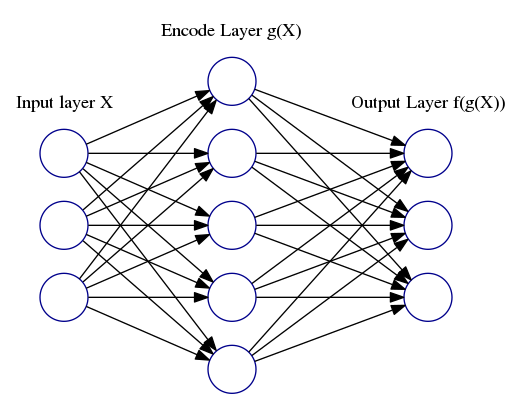
\includegraphics[scale=0.4]{parts/res/autoencoder.png}}
  \caption{Auto-Encoder}
  \label{fig:AE}
\end{figure}
\subsection{Background knowledge}
The background knowledge are pairwise constraints :
\begin{itemize}
\item \textbf{Must-link} constraint $ML$ : $(X, X') \in ML \implies $ X and X' are in the
  same cluster.
\item \textbf{Cannot-link} constraint $CL$ : $(X, X') \in CL \implies $ X and X' are in
  different cluster.
\end{itemize}
A first method to integrate pairwise constraints to the K-Means is to use the 
COP-KMeans algorithm introduced by Wagstaff\cite{Wagstaff:2001:CKC:645530.655669}.
In this algorithm, we assign each document to the closest cluster(see algorithm~\ref{algo:cop}), 
which did not violate ML and CL constraints (see algorithm~\ref{algo:vio}).
\begin{algorithm}[!h]
  \SetKwInOut{Input}{input}
  \SetKwInOut{Output}{output}
  \Input{Corpus C, must-link constraints $ML \subseteq C x C$,
    cannot-link constraints $CL \subseteq C x C$}
  \Output{Clusters $S_1, S_2, ..., S_k$}
  Let $S_1, S_2 , ..., S_k$ be the initial clusters\\
  \Repeat{Convergence}{
    \ForEach{$X_i \in C$}{
      Assign $X_i$ to closest $S_j$ such that Violate-Constraints($X_i, C_j, CL,
      ML$) is false.\\
      \If{No such clusters exists}{
        return \{\}\\
      }
    }
    \ForEach{Clusters $S_i$}{
      Update centroids.\\
    }
  }
  \Return{$S_1, S_2, ..., S_k$}
  \caption{\label{algo:cop}COP-Kmeans}
\end{algorithm}
\begin{algorithm}[!h]
  \SetKwInOut{Input}{input}
  \SetKwInOut{Output}{output}
  \Input{Ducument X, Clusters S, must-link constraints $ML \subseteq C x C$,
    cannot-link constraints $CL \subseteq C x C$}
  \Output{True if constraints are violate, False otherwise}
  \ForEach{($X, X' \in ML$)}{
    \If{$X' \in S$}{
      \Return{True}
    }
  }
  \ForEach{($X, X' \in CL$)}{
    \If{$X' \in S$}{
      \Return{True}
    }
  }
  \Return{False}
  \caption{\label{algo:vio}Violate-Constraints}
\end{algorithm}
Another method, proposed by Hsu and Kira \cite{2015arXiv151106321H}, consists to 
use a neural Network based end-to-end clustering framework. This network 
directly assigns clusters in the output layer. Then they use the softmax 
function on the output layer and the KL-Divergence to learn a latent space 
which minimizes the statistical distance between predicted cluster probabilities 
for similar pairs while maximizing the distance for dissimilar pairs

\begin{equation}
  P = f(x_p), ~ Q = f(x_q)
\end{equation}

\begin{equation}
  KL(P||Q) = \sum_i^k P_ilog\frac{P_i}{Q_i}
\end{equation}

\begin{equation}
  I_s = \left\{
\begin{array}{ll}
  1 & \mbox{if $x_p$ and $x_q$ is a similar pair}\\
  0 & \mbox{Otherwise.}
\end{array}
\right.
\end{equation}
%
\begin{equation}
  I_{ds} = \left\{
\begin{array}{ll}
  1 & \mbox{if $x_p$ and $x_q$ is a dissimilar pair}\\
  0 & \mbox{Otherwise.}
\end{array}
\right.
\end{equation}
\begin{equation}
  Loss(P || Q) = I_s(x_p, x_q)KL(P || Q) + I_{ds}(x_p, x_q)max(0,
  \eta-KL(P||Q))
\end{equation}
\begin{equation}
  L(P,Q) = Loss(P || Q) + Loss(Q || P)
\end{equation}
\subsection{\label{seq:DeepClust}Deep Clustering}
A several approaches for the deep $K$-Means propose to jointy learn the
representation and perform the $K$-Means algorithm \cite{2018arXiv180107648A}.
In these approaches, network's loss is divided in two parts :
\begin{itemize}
\item \textbf{Non-Clustering loss} : The non-clustering loss does not
  take into account of the clustering parts. In general, the non-clustering 
  loss is the reconstruction loss of the auto-encoder. We can add additional 
  information in the non-clustering loss to biais the representation. For
  example, in our case, we add penalties to integrate lexical constraints
  and pairwise constraints.
\item \textbf{Clustering loss} : The clustering loss allows to learn a
  $K$-means friendly representation.
\end{itemize}
The loss function takes the form :
\begin{equation}
L(X;\theta) = \lambda L_{NonClust}(C;\theta) + (1-\lambda)L_{Clust}(C; \theta)
\end{equation}
Where $\lambda \in [0 ; 1]$ is a constant specifying the weighting between both 
functions.
It is an additional hyperparameter for the network training.\\
Moradi Fard, Thonet and Gaussier \cite{Deap-K-Means} proposed a method for deep $K$-Means 
clustering based on a continuous reparametrization of the objective function 
that leads to a truly joint solution. 
The problem takes the form : 
\begin{equation}
L(C ,\beta;\theta,R) = L_{NonClust}(C;\theta,R ) + \lambda L_{Clust}(C,\beta;\theta,R)
\end{equation}
\begin{equation}
L_{NonClust}(C;\theta,R ) = \sum_{X \in C} ||X - f(g(X;\theta))||_2^2
\end{equation}
\begin{equation}
\begin{aligned}
  L_{Clust}(C,\beta;\theta,R) = \sum_{X \in C}F(g(X),c(g(X, \theta); R))\\
  F(g(X),c(g(X, \theta); R)) = ||g(X) - c(g(X, \theta); R) ||_2^2\\
  c(g(X; \theta); R) = \argmin_{k = 1 .. K} || X - r_k||_2^2
\end{aligned}
\end{equation}
$F(g(X),c(g(X, \theta); R))$ is a differentiable distance function.
$c(X ; R)$ is a non differentiable function that assigns the document X
to its nearest centroid.\\
They transform this representation as follows :
\begin{equation}
L_{Clust} = \sum_{X \in C}\sum_{k=1}^K F(g(X; \theta), r_k) G_{k, F}(g(X; \theta), \beta; R)
\end{equation}
where $G_{k, F}$ is a differentiable function such that :
\begin{equation}
  \lim\limits_{\beta \rightarrow \beta_0}G_{k, F}(g(X; \theta), \beta; R) = \left\{
\begin{array}{ll}
  1 & \mbox{if} r_k = c(g(X, \theta); R)\\
  0 & \mbox{Otherwise.}
\end{array}
\right.
\end{equation}
where $\beta$ play the role of an inverse temperature. In \cite{Deap-K-Means}
, $G_{k,F}$ was chosen to be a parameterized softmax : 
$G_{k, F}(g(X; \theta), \beta; R) = \frac{e^{-\beta F(g(X, \theta),r_k)}}
{\sum_{k' = 1}^K e^{-\beta F(g(X, \theta),r_k')}}$\\
To update $(\theta, R)$, they used the stochastic gradient descent (SGD)
as follows :
\begin{equation}
  (\theta, R) \gets (\theta, R) - \epsilon \frac{1}{|\widetilde{C}|}
  \nabla_{(\theta, R)} L(C, \beta; \theta, R)
\end{equation}
where $\widetilde{C}$ is a random mini batch of C, and $\epsilon$ the
learning rate.
Algorithm \ref{algo:dkm} summarizes the deep k-Means algorithm :
\begin{algorithm}[!h]
  \SetKwInOut{Input}{input}
  \SetKwInOut{Output}{output}
  \Input{Corpus C , number of clusters K, balancing parameter $\lambda$,
    scheme for $\beta$, number of epochs T ,
    number of minibatches MB , learning rate $\epsilon$}
  \Output{Auto-Encoder parameter $\theta$, cluster representative R}
  Initialise $\theta$ and $r_k$, $1 \leq k \leq K$ (randomly or through 
  pretraining)\\
  \ForEach{$\beta = m_\beta : M_\beta$}{
    \ForEach{t = 1 : T}{
      \ForEach{n = 1 : MB}{
        Draw minibatch $\widetilde{C} \subseteq  C$\\
        Update ($\theta, R$) using SGD
      } 
    }  
  }
  \caption{\label{algo:dkm}Deep $K$-Means}
\end{algorithm}
